\chapter{Kontrollieren}

\section{Testprotokoll}
Dieser Abschnitt protokolliert das Testkonzept (siehe Kapitel \ref{sec:testkonzept}).
\subsection{Manuelle Tests}
\label{sec:automated-tests}

\subsection{Automatisierte Tests}
\label{sec:manual-tests}
Die automatisierten Tests wurden mit MiniTest und Capybara geschrieben, wie von Redmine selbst
vorgegeben. Auch das laufen lassen der Tests basiert auf dem vom Redmine vorgegebenen Rake Task. Um die
Tests laufen zu lassen, muss man \bgmintinline{bash}{rake redmine:plugins:test NAME=gnosis} im Terminal
ausführen. Dabei wird der Name des Plugins angegeben, damit nur die Tests für dieses Plugin laufen. Im
\bgmintinline{bash}{bin} Verzeichnis befindet sich eine \bgmintinline{bash}{bin/test} Datei, welche
diesen Rake Task ausführt und den Output schön formatiert.
Der Output sieht dann ungefähr so aus:
\begin{center}
    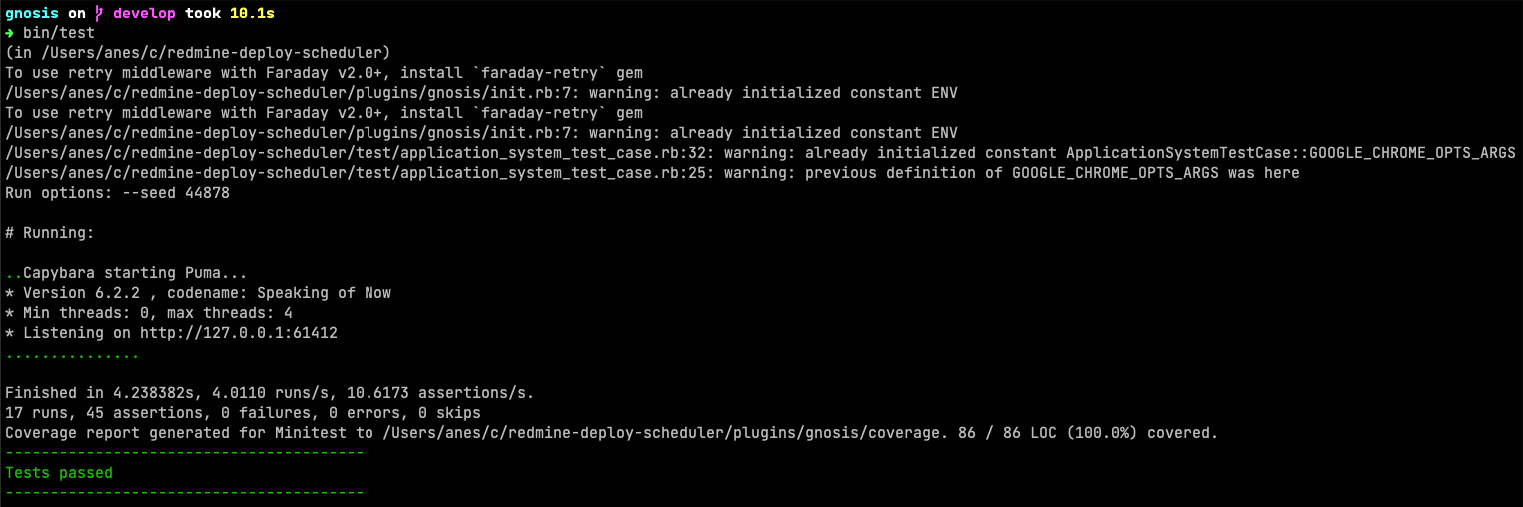
\includegraphics[width=0.75\textwidth]{images/misc/simplecov_terminal_output.png}
    \label{fig:simplecov_terminal_output}
\end{center}

\section{Versionierung}
\subsection{Dokumentation}
\subsection{Programm}
\subsubsection{Selbstkritische PR Reviews}

\section{Kopplung vom Hauptprogramm}

